\section{Auswertung}
\label{sec:Auswertung}

Im folgenden wird mit den Konstanten 
\begin{align*}
  h = 4,136 \cdot 10^{-15} \; eVs\\
  c = 2,99 \cdot 10^8 \; m/s \\
  d = 201,4 \cdot 10^{-12}\; m \\
\end{align*}

gerechnet. $h$ ist das Planck'sche Wirkungsquantum, $c$ die Lichtgeschwindigkeit,
$d$ die Gitterkonstante des Lithium-Flourid-Kristalls.\\
Die Beugungsordnung $n$ beträgt $n = 1$.




\subsection{Emissionsspektrum von Kupfer}
\label{subsec:spektrumCU}


In \autoref{fig:emissionssp} ist das Bremsspektrum der Röntgenstrahlung, die auf das Kupfer trifft, zu sehen.\\
Es wird die Zählrate $N$ der Impulse pro Sekunde gegen die Wellenlänge $\lambda$ in Metern aufgetragen.\\

\begin{figure}
  \centering
  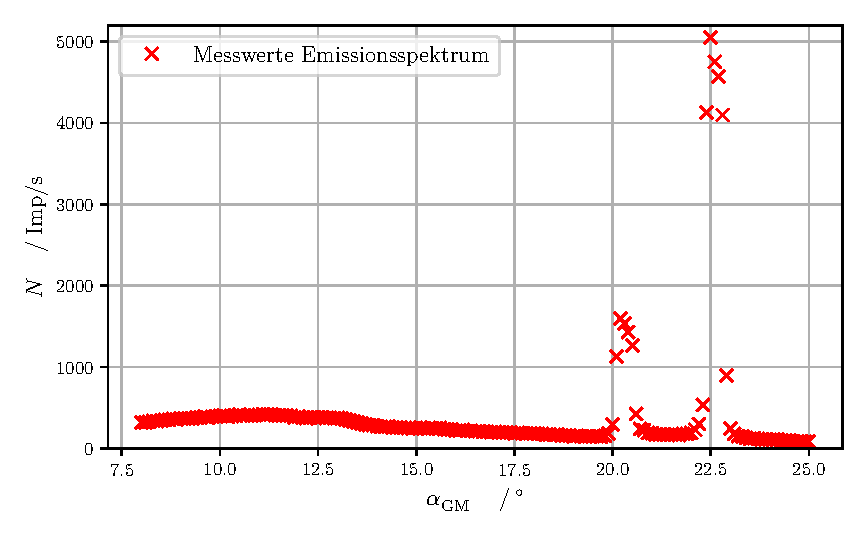
\includegraphics{build/emissionsspektrum.pdf}
  \caption{Das Emissionsspektrum von Kupfer mit gekennzeichneten Peaks. Der erste Peak stellt $K_{\beta}$ dar, der zweite $K_{\alpha}$.}
  \label{fig:emissionssp}
\end{figure}

Es sind die Peaks $K_{\alpha}$ und $K_{\beta}$ bei den Winkeln $\alpha(K_{\alpha})= 22,5°$ 
und $\alpha(K_{\beta}) = 20,02°$ zu erkennen.\\

Mit Hilfe der Formel ----- lassen sich die zu den Peaks gehörigen Energien
\begin{align*}
  E(K_{\alpha}) = (8043 \pm 34) eV \\
  E(K_{\beta}) = (8910 \pm 40) eV
\end{align*}





\subsection{Transmission $T$ des Aluminiumabsorbers}
\label{subsec:transmission}

Die Funktion der Transmisson $T(\lambda)$ beschreibt die Transmission der 
Röntgenstrahlung durch die Aluminiumplatte des Aufbaus in Abhängigkeit von der Wellenlänge.\\

Es wird die Totzeit $\tau$ des Geiger-Müller-Zählrohrs als $\tau = 90 \cdot 10^{-6}$ angenommen. Die 
Integrationszeit der einzelnen Messungen lautet $t = 200s$. \\
Es gilt der Fehler $\Delta N = \frac{\sqrt{N \cdot t}}{t}$.\\


\begin{figure}
  \centering
  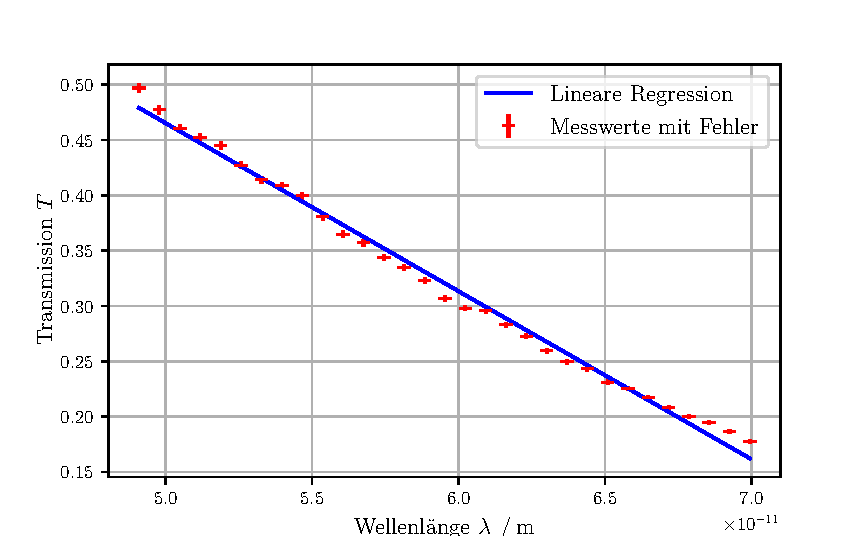
\includegraphics{build/transmission.pdf}
  \caption{Die Transmission $T$ in Abhängigkeit der Wellenlänge $\lambda$ mit linearer Ausgleichsgeraden.}
  \label{fig:transm}
\end{figure}

Die Ausgleichsgerade in \autoref{fig:transm} hat eine Gleichung der Form $T(\lambda) = a \cdot \lambda + b$ mit 
den Parametern $a = (-1,519 \pm 0,024)\cdot 10^{10} m^{-1}$ und $b = 1,225 \pm 0,014$.

\begin{figure}
  \centering
  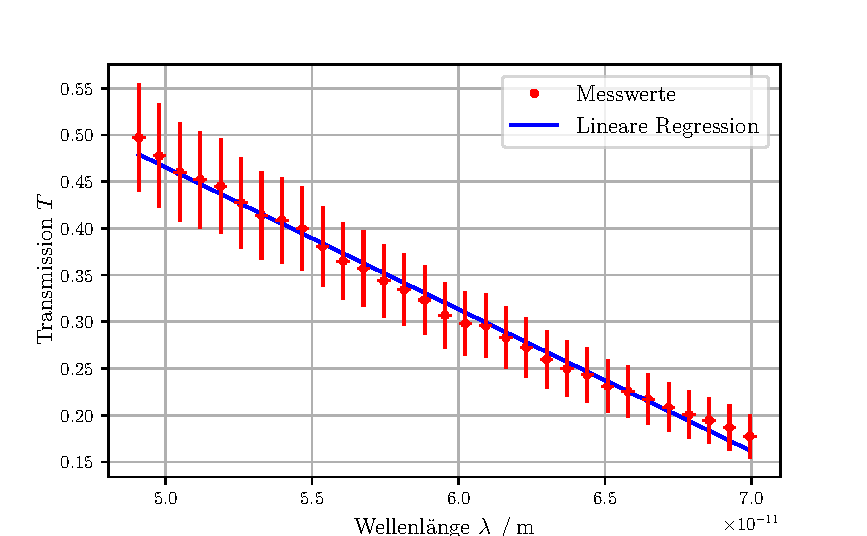
\includegraphics{build/transmission2.pdf}
  \caption{Die Transmission $T$ in Abhängigkeit der Wellenlänge $\lambda$ mit linearer Ausgleichsgeraden und Fehlerbalken.}
  \label{fig:transm2}
\end{figure}



\subsection{Ermittlung der Compton-Wellenlänge}
\label{subsec:comptonwellenl}

Die Intensität $I_0 = 2731 \pm 50$ wird ohne Absorber, $I_1 = 1180 \pm 34$ und $I_2 = 1024 \pm 32$ mit Aluminiumabsorber zwischen Röntgenröhre
und Plexiglas-Streuer bzw. zwischen Plexiglas-Streuer und Geiger-Müller-Zählrohr gemessen.\\
Die dazugehörige Integrationszeit beträgt $t = 300s$.\\

Aus den Intensitäten lassen sich die Transmissionen der Aufbauten mit $-----$ berechnen. \\
Diese ergeben sich zu $T_1 = 0,423 \pm 0,015$ und $T_2 = 0,375 \pm 0,014$.\\

Schleißlich wird die Compton-Wellenlängen $\lambda_C$ aus den Transmissionen und den Parametern der Ausgleichsgerade 
in \autoref{fig:transm} bestimmt. \\
Mit 
\begin{align*}
  \lambda = \frac{T-b}{a}
\end{align*}
ergeben sich
\begin{align*}
  \lambda_1 = (52,2 \pm 1,6) \cdot 10^{-12}m \\
  \lambda_2 = (55,9 \pm 1,6) \cdot 10^{-12}m,
\end{align*}
sodass die Compton-Wellenlänge sich auf $\lambda_C = \lambda_2 - \lambda_1 = (3,8 \pm 1,1) \cdot 10^{-12}m$ beläuft.\\